% Wilson Line for SIDIS TMD PDF (Conceptual)
\documentclass[tikz]{standalone}
\usepackage{tikz}
\usetikzlibrary{decorations.pathmorphing, arrows.meta, patterns, calc, positioning}
\usetikzlibrary{decorations.markings}

\usepackage{amsmath,amssymb}

% \begin{document}
% \begin{tikzpicture}[
%     scale=1.5,
%     every node/.style={transform shape},
%     % Light-cone directions
%     lcplus/.style={->, thick, blue!70!black, >=Latex}, lcminus/.style={->, thick, red!70!black, >=Latex},
%     % Wilson line style
%     wilson/.style={line width=1.5pt, draw=green!50!black, postaction={decorate, decoration={markings,mark=at position 0.5 with {\arrow{>}}}}},
%     wilson_staple/.style={line width=1.5pt, draw=green!50!black, dashed, postaction={decorate, decoration={markings,mark=at position 0.5 with
%                   {\arrow{>}}}}}, ]

%   % Coordinates for psi-bar and psi fields
%   \coordinate (psi_bar_pos) at (0,0);
%   \coordinate (psi_pos) at (2,0.5); % xi_T separation

%   % Label for xi^- (light-cone time/longitudinal separation)
%   \draw[<->, gray] ($(psi_pos) + (0.2,0)$) -- ($(psi_pos) + (0.2,-1.5)$) node[midway, right, black] {$\xi^-$ (LC time)};
%   \node at ($(psi_pos) + (0,-1.5)$) {}; % Anchor for xi- direction

%   % Light-cone axes (conceptual)
%   \draw[lcplus] (-1, -1.8) -- (1, -1.8) node[right] {$n^+$ (e.g., $P^+$ direction)};
%   \draw[lcminus] (-1.5, -1) -- (-1.5, 1) node[above] {$n^-$ (e.g., to $-\infty$)};

%   % Quark fields
%   \node[fill=blue!20, circle, inner sep=2pt] at (psi_bar_pos) {$\bar{\psi}(0)$};
%   \node[fill=red!20, circle, inner sep=2pt] at (psi_pos) {$\psi(\xi)$};
%   \node[below right=0.1cm of psi_pos, black] {$\xi = (0, \xi^-, \vec{\xi}_T)$};

%   % Wilson line staple for SIDIS TMD PDF (future-pointing for FSI)
%   % Path: xi -> +infinity (along n-) -> transverse link -> +infinity (along n-) -> 0
%   \coordinate (xi_inf_staple_start) at ($(psi_pos) + (-0.5, 1.5)$); % Point at +infinity along n-
%   \coordinate (zero_inf_staple_end) at ($(psi_bar_pos) + (-0.5, 1.5)$); % Point at +infinity along n-

%   \draw[wilson_staple, green!70!black] (psi_pos) -- ($(psi_pos)!(xi_inf_staple_start)!(psi_pos)$) -- (xi_inf_staple_start) node[pos=0.7, above, sloped, black!70!green] {$W[\xi, +\infty_{n^-}]$};
%   \draw[wilson_staple, green!70!black] (xi_inf_staple_start) -- (zero_inf_staple_end) node[midway, above, black!70!green] {$W_{transverse}(+\infty_{n^-})$};
%   \draw[wilson_staple, green!70!black] (zero_inf_staple_end) -- ($(psi_bar_pos)!(zero_inf_staple_end)!(psi_bar_pos)$) -- (psi_bar_pos) node[pos=0.3, above, sloped, black!70!green] {$W[+\infty_{n^-}, 0]$};

%   % Direct Wilson line (often part of the full structure, or for comparison)
%   % \draw[wilson, opacity=0.3] (psi_pos) to[bend left=10] (psi_bar_pos) node[midway, below, sloped, black!70!green, opacity=0.7] {$W[\xi,0]$ (direct)};

%   % Labels and annotations
%   \node[text width=5cm, align=center, below left=0.5cm of psi_bar_pos, black] at (1, -2.5) {
%     Conceptual Wilson line for SIDIS TMD PDF.\newline
%     Future-pointing staple (dashed green) represents final-state interactions.
%     Path: $\xi \xrightarrow{n^-} +\infty_{n^-} \xrightarrow{\text{transverse}} +\infty_{n^-} \xrightarrow{n^-} 0$.
%   };

%   % Indicate transverse plane (conceptually)
%   \draw[gray, dashed] (-0.5, -0.25) ellipse (0.5cm and 0.2cm);
%   \node[gray] at (-1.2, -0.25) {$\vec{\xi}_T$ plane};

% \end{tikzpicture}
% \end{document}

\begin{document}
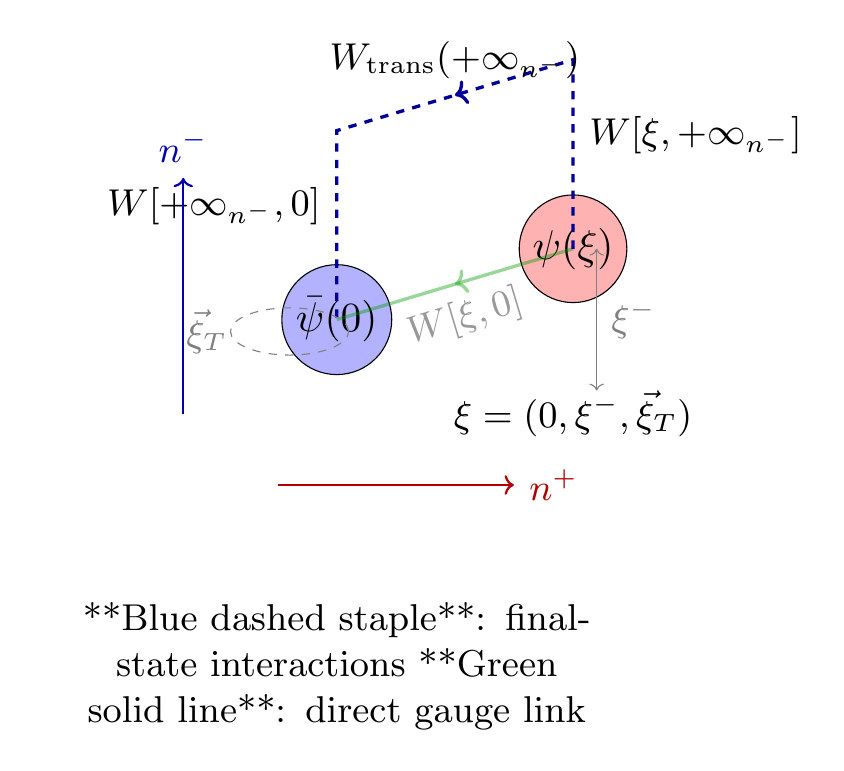
\begin{tikzpicture}[
    scale=1.5,
    every node/.style={transform shape},
    % Styles
    wilson/.style={ line width=1.2pt, draw=green!60!black, postaction={decorate, decoration={ markings, mark=at position 0.5 with {\arrow{>}} }} },
    staple/.style={ line width=1.2pt, draw=blue!60!black, dashed, postaction={decorate, decoration={ markings, mark=at position 0.5 with {\arrow{>}} }}
      }, field/.style={circle, draw, fill=#1!30, inner sep=1.5pt}, label/.style={font=\small}, ]

  % 1) Quark fields
  \coordinate (O) at (0,0);
  \coordinate (X) at (2,0.6);

  \node[field=red]  (psiX) at (X) {$\psi(\xi)$};
  \node[field=blue] (psi0) at (O) {$\bar\psi(0)$};

  % 2) Direct Wilson line (straight gauge link)
  \draw[wilson, opacity=0.4]
  (X) -- (O)
  node[midway, below, sloped, label] {$W[\xi,0]$};

  % 3) Staple path: xi -> +∞ (n⁻) -> transverse → +∞ (n⁻) → 0
  %    we choose n⁻ along +y, transverse along –x
  \coordinate (A) at ($(X) + (0,1.6)$);    % xi → +∞ᶰ⁻
  \coordinate (B) at ($(O) + (0,1.6)$);    % transverse at +∞ᶰ⁻

  \draw[staple]
  (X) -- (A) node[pos=0.6, right,  label] {$W[\xi,+\infty_{n^-}]$}
  -- (B) node[midway, above,    label] {$W_{\rm trans}(+\infty_{n^-})$}
  -- (O) node[pos=0.4, left,     label] {$W[+\infty_{n^-},0]$};

  % 4) Labels for light‐cone directions
  \draw[->, thick, red!70!black]  (-0.5,-1.4) -- (1.5,-1.4) node[right,label] {$n^+$};
  \draw[->, thick, blue!70!black] (-1.3,-0.8) -- (-1.3, 1.2) node[above,label] {$n^-$};

  % 5) Separation and coordinate box
  \draw[<->, gray]
  ($(X)+(0.2,0)$) -- ($(X)+(0.2,-1.2)$)
  node[midway, right,label] {$\xi^-$};
  \node[label] at ($(X)+(0.0,-1.4)$)
  {$\xi=(0,\xi^-,\vec\xi_T)$};

  % 6) Transverse‐plane ellipse
  \draw[gray,dashed] (-0.4,-0.1) ellipse (0.5cm and 0.2cm);
  \node[gray,label] at (-1.1,-0.1) {$\vec\xi_T$};

  % 7) Caption
  \node[text width=5cm, align=center, below=1.8cm of psi0, label]{
    **Blue dashed staple**: final‐state interactions
    **Green solid line**: direct gauge link
  };
\end{tikzpicture}
\end{document}